% Template for IGARSS-2018 paper; to be used with:
%          spconf.sty  - LaTeX style file, and
%          IEEEbib.bst - IEEE bibliography style file.
% --------------------------------------------------------------------------
\documentclass{article}
\usepackage{spconf,amsmath,epsfig,graphicx}
\usepackage{subcaption}
\usepackage[noend]{algpseudocode}
\usepackage{algorithm}
\usepackage{caption}


% Example definitions.
% --------------------
\def\x{{\mathbf x}}
\def\L{{\cal L}}

% Title.
% ------
\title{Extracting linear routes from heatmaps. An AIS Case Study in Europe.}
%
% Single address.
% ---------------
\name{T.L. Grobler$^{\dagger}$ and W. Kleynhans$^{\star}$}
\address{$\dagger$Dept of Mathematical Sciences, Computer Science Division, Stellenbosch University,\\ Private Bag X1, 7602 Matieland, South Africa\\
$\star$XXX}
%
% For example:
% ------------
%\address{School\\
%	Department\\
%	Address}
%
% Two addresses (uncomment and modify for two-address case).
% ----------------------------------------------------------
%\twoauthors
%  {A. Author-one, B. Author-two\sthanks{Thanks to XYZ agency for funding.}}
%	{School A-B\\
%	Department A-B\\
%	Address A-B}
%  {C. Author-three, D. Author-four\sthanks{The fourth author performed the work
%	while at ...}}
%	{School C-D\\
%	Department C-D\\
%	Address C-D}
%
\begin{document}
%\ninept
%
\maketitle
%
\begin{abstract}
In this paper we present a heat-map segmentation algorithm. The proposed segmentation algorithm
segments a heat-map into high traffic regions and low traffic regions. The borders of the different regions often coincide with high traffic routes. We then test the proposed 
algorithm on a heat-map constructed from Automatic Identification System (AIS) data collected in the Celtic sea, the Channel and the Bay of Biscay. The results show that the approach shows promise and if improved further 
it could become a viable segmentation strategy.
\end{abstract}
%
\begin{keywords}
Principal Component Analhysis (PCA), dimensionality reduction, harmonic analysis, time-series, Moderate Resolution Imaging Spectroradioameter (MODIS).
\end{keywords}
\begin{abstract}
\end{abstract}


Often, when we first inspect a dataset containing the temporal-spatial coordinates of multiple objects (i.e. the movements of say humans, animals or vessels)
we would create a heat-map (grid data onto a two-dimensional grid) so that we can build some intuition (gather information) about the data.
The information we extract from heat-maps (insight gained) can then be used to further analyze the original data. Some examples of the useful kind of information which can be extracted from a 
heat-map include: high traffic volume routes and regions. In this paper, we present an automatic heat-map segmentation algorithm which will allow us to automatically extract the 
 aforementioned pieces of information. In this paper we focus primarily on AIS data (shipping data). 
 
The pseudo-code of the proposed segmentation algorithm is given in Algorithm 1. 

\begin{algorithm}
 \caption{Polygon Heat-map Segmentation Algorithm}\label{euclid}
 \begin{algorithmic}[1]
 \Procedure{polygonSegmentation}{heatmap,coastlinemask,landmask}
 \State $\textrm{heatmap} \gets \log(\textrm{heatmap}+1)$
 \Comment{emphasizes the linear tracks}
 \State $\textrm{copy} \gets \textrm{heatmap}$
 \Comment{store a copy of original}
 \State $\textrm{heatmap} \gets \textrm{maskCoastline(heatmap,coastlinemask)}$
 \Comment{mask coastline}
 \State $\textrm{heatmap} \gets \textrm{heatmap - medianFilter(heatmap)}$ 
 \Comment{detect outliers}
 \State $\textrm{heatmap} \gets \textrm{otsuThreshold(heatmap)}$
 \Comment{binary segmentation}
 \State $\textrm{heatmap} \gets \textrm{binaryOpening(heatmap)}$
 \Comment{clears the noisy region}
 \State $\textrm{lines} \gets \textrm{houghTransform(heeatmap)}$
 \Comment{extract lines from image}
 \State $\textrm{polygons} \gets \textrm{polygonize(lines,coastlinemask,landmask)}$
 \Comment{polygonize}
 \For{polygon in polygons}
     \State $\textrm{heatmap[polygon]} \gets \textrm{average(copy[polygon])}$ 
 \EndFor
 \State $\textrm{heatmap[coastlinemask]} \gets \textrm{average(copy[polygon])}$
 \State $\textrm{heatmap[landmask]} \gets 0$
 \Comment{segmentation}
 \State plot(heatmap)
 
% \State $\textit{stringlen} \gets \text{length of }\textit{string}$
% \State $i \gets \textit{patlen}$
% %\BState \emph{top}:
% \If {$i > \textit{stringlen}$} \Return false
% \EndIf
% \State $j \gets \textit{patlen}$
% %\BState \emph{loop}:
% \If {$\textit{string}(i) = \textit{path}(j)$}
% \State $j \gets j-1$.
% \State $i \gets i-1$.
% \State \textbf{goto} \emph{loop}.
% \State \textbf{close};
% \EndIf
% \State $i \gets i+\max(\textit{delta}_1(\textit{string}(i)),\textit{delta}_2(j))$.
% \State \textbf{goto} \emph{top}.
 \EndProcedure
 \end{algorithmic}
 \end{algorithm}
 
In this paper we present a heat-map segmentation algorithm. The proposed segmentation algorithm
segments a heat-map into high traffic regions and low traffic regions. The borders of the different regions often coincide with high traffic routes. We then test the proposed 
algorithm on a heat-map constructed from Automatic Identification System (AIS) data collected in the Celtic sea, the Channel and the Bay of Biscay. The results show that the approach shows promise and if improved further 
it could become a viable segmentation strategy.
 
The first step of the algorithm is to take the elment-wise logarithm of the heat-map passed into it as an argument. This visually emphasises the high volume routes found within the heat-map. We then 
create a binary image. To achieve this we first filter the logged heat-map. We make use of a median filter as it is well known for its ability to detect outliers. We then threshold (we used Otsu thresholding) the  
filtered heat-map. To clean the binary heat-map (we obtained by applying thresholding) we apply the morphological opening operator to it (which is used to remove noise from the foreground).
We then use the Hough Transform to extract the longer lines from the opened binary heat-map. We then polygonize the heat-map using the extracted lines. We can then 
segment the original heat-map into different regions using the aforementioned derived polygons. The result of applying the above algorithm to AIS data is depicted in Figure~\ref{fig7}.


Figure~\ref{fig7} highlights some of the shortcomings of this segmentation strategy. The Hough-Transform struggles to detect all 
the lines. It especially struggles with short and closely spaced parallel lines (can be mitigated by iteratively applying the algorithm to each segmented region). It works on the assumption that straight line routes were followed (which is not guaranteed). Some of the line segments should also be removed prior to polygonization as they do not 
represent true high volume routes. The value of the coastline segments can be separately computed within each polygon.
 
\begin{figure*}[h] 
  \begin{subfigure}[b]{0.5\linewidth}
    \centering
    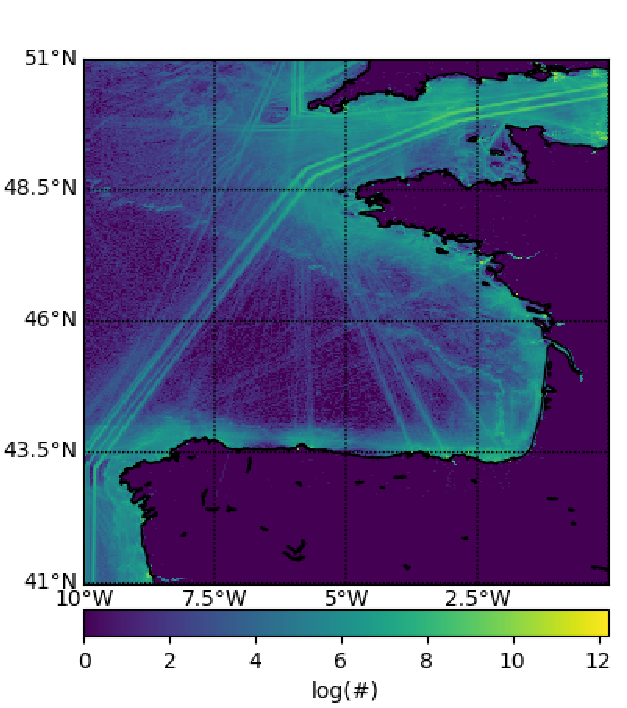
\includegraphics[width=0.8\linewidth]{CELTICcrop.pdf} 
    \caption{Logarithm applied} 
    \label{fig7:a} 
    \vspace{4ex}
  \end{subfigure}%% 
  \begin{subfigure}[b]{0.5\linewidth}
    \centering
    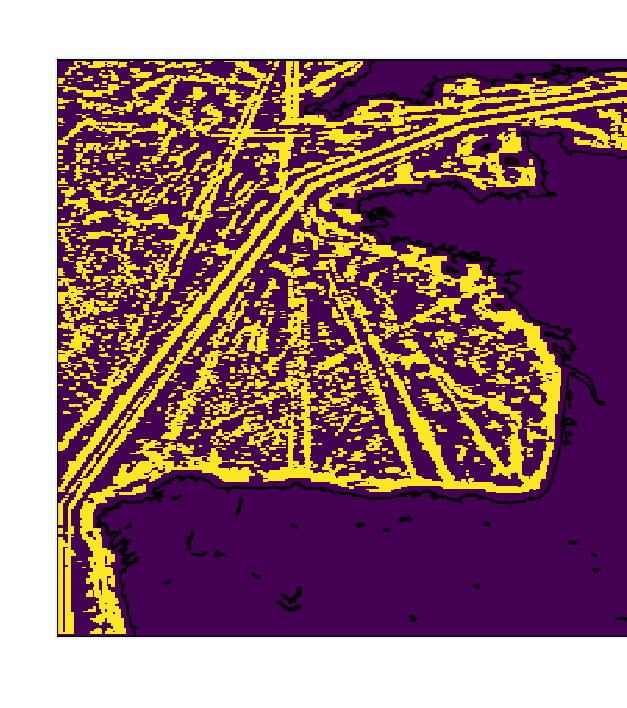
\includegraphics[width=0.8\textwidth]{CELTICopened-crop.pdf} 
    \caption{Binary segmented image} 
    \label{fig7:b} 
    \vspace{4ex}
  \end{subfigure} 
  \begin{subfigure}[b]{0.5\linewidth}
    \centering
    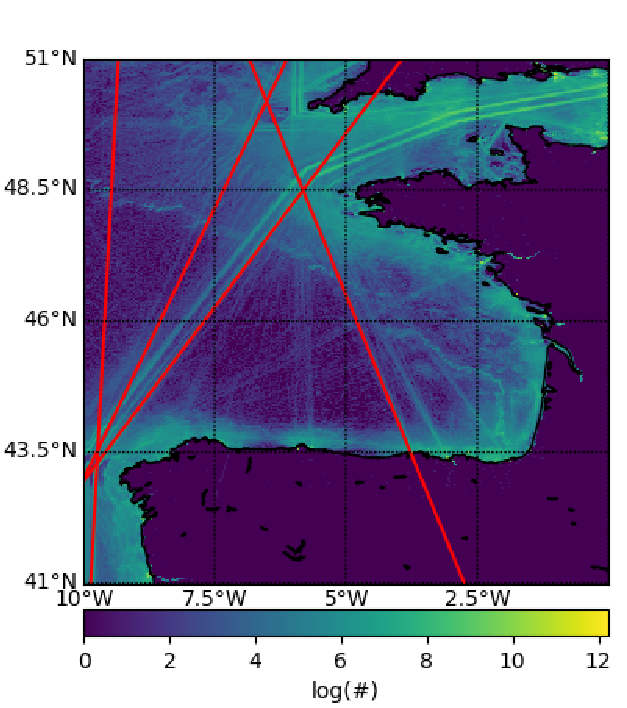
\includegraphics[width=0.8\textwidth]{CELTIClines-crop.pdf} 
    \caption{Hough Transform} 
    \label{fig7:c} 
  \end{subfigure}%%
  \begin{subfigure}[b]{0.5\linewidth}
    \centering
    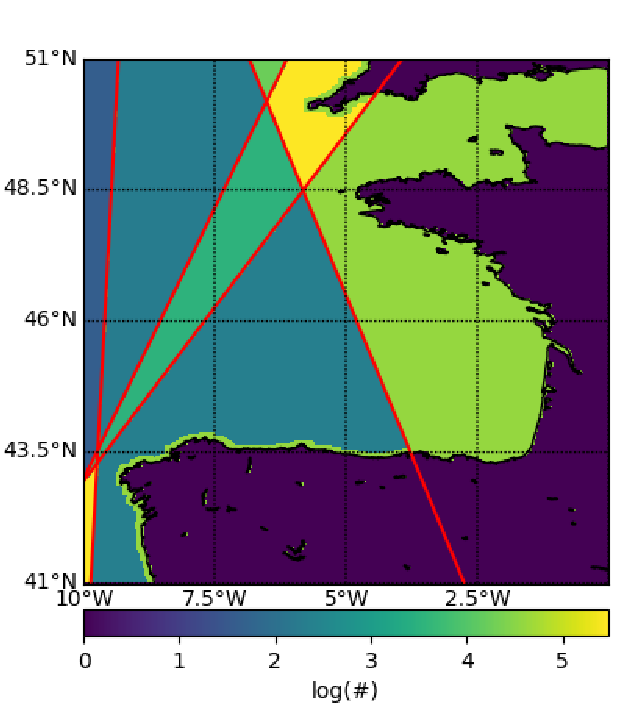
\includegraphics[width=0.8\textwidth]{CELTICsegmented-crop.pdf} 
    \caption{Segmented image} 
    \label{fig7:d} 
  \end{subfigure} 
  \caption{A heat-map of AIS ship positions within the Celtic sea, the Channel and the Bay of Biscay (France) [Longitude between $-10^{\circ}$ and $0^{\circ}$ and Latitude between $45^{\circ}$ and $51^{\circ}$]. The above subfigures were generated by applying the segmentation algorithm depicted in Algorithm 1 to an existing heat-map of the region. The top left image was optained after the logarithm of the original heat-map was taken (element-wise). The top right image 
  was obtained by applying binary thresholding and morphological opening to a filtered variant of the top left heat map. The right bottom heat-map depicts the lines we were able to extract 
  from the top right image using the Hough Transform. The bottom right image contains the final segmented heat map. Notice that the coastline is segmented separately.}
  \label{fig7} 
\end{figure*}

...

% \section{Introduction}
% \label{sec:intro}
% 
% These guidelines include complete descriptions of the fonts, spacing, and
% related information for producing your proceedings manuscripts. Please follow
% them and if you have any questions, direct them to Conference Management
% Services, Inc.: Phone +1-979-846-6800 or Fax +1-979-846-6900 or email
% to \verb+papers@igarss2018.org+.
% 
% \section{Formatting your paper}
% \label{sec:format}
% 
% All printed material, including text, illustrations, and charts, must be kept
% within a print area of 7 inches (178 mm) wide by 9 inches (229 mm) high. Do
% not write or print anything outside the print area. The top margin must be 1
% inch (25 mm), except for the title page, and the left margin must be 0.75 inch
% (19 mm).  All {\it text} must be in a two-column format. Columns are to be 3.39
% inches (86 mm) wide, with a 0.24 inch (6 mm) space between them. Text must be
% fully justified.
% 
% \section{PAGE TITLE SECTION}
% \label{sec:pagestyle}
% 
% The paper title (on the first page) should begin 1.38 inches (35 mm) from the
% top edge of the page, centered, completely capitalized, and in Times 14-point,
% boldface type.  The authors' name(s) and affiliation(s) appear below the title
% in capital and lower case letters.  Papers with multiple authors and
% affiliations may require two or more lines for this information.
% 
% \section{TYPE-STYLE AND FONTS}
% \label{sec:typestyle}
% 
% To achieve the best rendering in the proceedings, we
% strongly encourage you to use Times-Roman font.  In addition, this will give
% the proceedings a more uniform look.  Use a font that is no smaller than nine
% point type throughout the paper, including figure captions.
% 
% In nine point type font, capital letters are 2 mm high.  If you use the
% smallest point size, there should be no more than 3.2 lines/cm (8 lines/inch)
% vertically.  This is a minimum spacing; 2.75 lines/cm (7 lines/inch) will make
% the paper much more readable.  Larger type sizes require correspondingly larger
% vertical spacing.  Please do not double-space your paper.  True-Type 1 fonts
% are preferred.
% 
% The first paragraph in each section should not be indented, but all the
% following paragraphs within the section should be indented as these paragraphs
% demonstrate.
% 
% \section{MAJOR HEADINGS}
% \label{sec:majhead}
% 
% Major headings, for example, "1. Introduction", should appear in all capital
% letters, bold face if possible, centered in the column, with one blank line
% before, and one blank line after. Use a period (".") after the heading number,
% not a colon.
% 
% \subsection{Subheadings}
% \label{ssec:subhead}
% 
% Subheadings should appear in lower case (initial word capitalized) in
% boldface.  They should start at the left margin on a separate line.
%  
% \subsubsection{Sub-subheadings}
% \label{sssec:subsubhead}
% 
% Sub-subheadings, as in this paragraph, are discouraged. However, if you
% must use them, they should appear in lower case (initial word
% capitalized) and start at the left margin on a separate line, with paragraph
% text beginning on the following line.  They should be in italics.
% 
% \section{PRINTING YOUR PAPER}
% \label{sec:print}
% 
% Print your properly formatted text on high-quality, 8.5 x 11-inch white printer
% paper. A4 paper is also acceptable, but please leave the extra 0.5 inch (12 mm)
% empty at the BOTTOM of the page and follow the top and left margins as
% specified.  If the last page of your paper is only partially filled, arrange
% the columns so that they are evenly balanced if possible, rather than having
% one long column.
% 
% In LaTeX, to start a new column (but not a new page) and help balance the
% last-page column lengths, you can use the command ``$\backslash$pagebreak'' as
% demonstrated on this page (see the LaTeX source below).
% 
% \section{PAGE NUMBERING}
% \label{sec:page}
% 
% Please do {\bf not} paginate your paper.  Page numbers, session numbers, and
% conference identification will be inserted when the paper is included in the
% proceedings.
% 
% \section{ILLUSTRATIONS, GRAPHS, AND PHOTOGRAPHS}
% \label{sec:illust}
% 
% % \begin{figure*}
% %   \begin{minipage}[b]{.48\linewidth}
% %   \centering
% %   \centerline{\includegraphics[width=0.45\linewidth]{./FFT1.pdf}}}
% %   \vspace{1.5cm}
% %   \centerline{(b) Results 3}\medskip
% % \end{minipage}
% % \hfill
% % \begin{minipage}[b]{0.48\linewidth}
% %   \centering
% %   \centerline{\includegraphics[width=0.45\linewidth]{./FFT1.pdf}}}
% %   \vspace{1.5cm}
% %   \centerline{(c) Result 4}\medskip
% % \end{minipage}
% % \end{figure*}
% 
% Illustrations must appear within the designated margins.  They may span the two
% columns.  If possible, position illustrations at the top of columns, rather
% than in the middle or at the bottom.  Caption and number every illustration.
% All illustrations should be clear wwhen printed on a black-only printer. Color
% may be used.
% 
% Since there are many ways, often incompatible, of including images (e.g., with
% experimental results) in a LaTeX document, below is an example of how to do
% this \cite{Lamp86}.
% 
% % Below is an example of how to insert images. Delete the ``\vspace'' line,
% % uncomment the preceding line ``\centerline...'' and replace ``imageX.ps''
% % with a suitable PostScript file name.
% % -------------------------------------------------------------------------
% 
% 
% % To start a new column (but not a new page) and help balance the last-page
% % column length use \vfill\pagebreak.
% % -------------------------------------------------------------------------
% %\vfill
% %\pagebreak
% 
% 
% \section{FOOTNOTES}
% \label{sec:foot}
% 
% Use footnotes sparingly (or not at all!) and place them at the bottom of the
% column on the page on which they are referenced. Use Times 9-point type,
% single-spaced. To help your readers, avoid using footnotes altogether and
% include necessary peripheral observations in the text (within parentheses, if
% you prefer, as in this sentence).
% 
% 
% \section{COPYRIGHT FORMS}
% \label{sec:copyright}
% 
% You must also electronically sign the IEEE copyright transfer
% form when you submit your paper. We {\bf must} have this form
% before your paper can be sent to the reviewers or published in
% the proceedings. The copyright form is provided through the IEEE
% website for electronic signature. A link is provided upon
% submission of the manuscript to enter the IEEE Electronic
% Copyright Form system.


\section{Conclusion}
\label{sec:ref}
We presented a feature extraction comparison framework in this paper. We demonstrated its usefulness by employing it and a case study to compare two feature extraction methods,
namely FFT and PCA. For the dataset we considered here we found that the PCA method performed on average 1.3 times better than the FFT method (across the spectral dimension).

%List and number all bibliographical references at the end of the paper.  The references can be numbered in alphabetic order or in order of appearance in the document.  When referring to them in the text, type the corresponding reference number in square brackets as shown at the end of this sentence \cite{C2}.

% References should be produced using the bibtex program from suitable
% BiBTeX files (here: strings, refs, manuals). The IEEEbib.bst bibliography
% style file from IEEE produces unsorted bibliography list.
% -------------------------------------------------------------------------
\bibliographystyle{IEEEbib}
\bibliography{strings,refs}

\end{document}
